%====================Step1====================%

%<*mtag100>
\begin{figure}[H]
\centering
\captionsetup{width=1\linewidth}
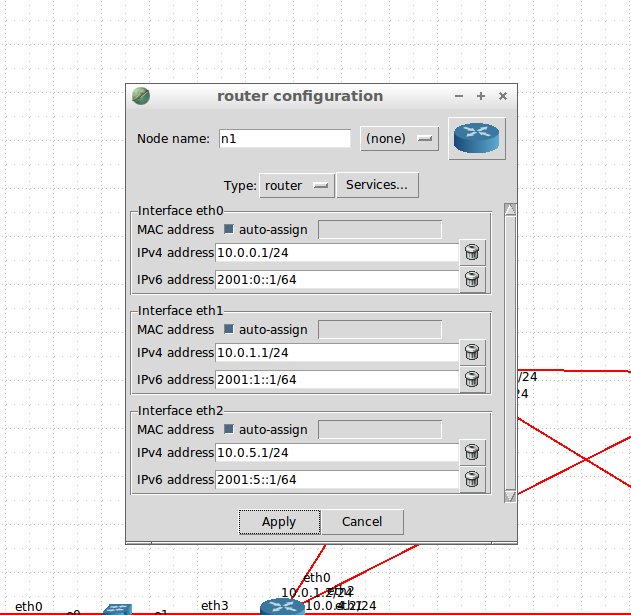
\includegraphics[scale=0.6]{\ImgPath/Ex4/Step1/services.png}
\caption{main configuration page}
\label{fig:1}
\centering
\end{figure}
%</mtag100>
%<*mtag101>
\begin{figure}[H]
\centering
\captionsetup{width=1\linewidth}
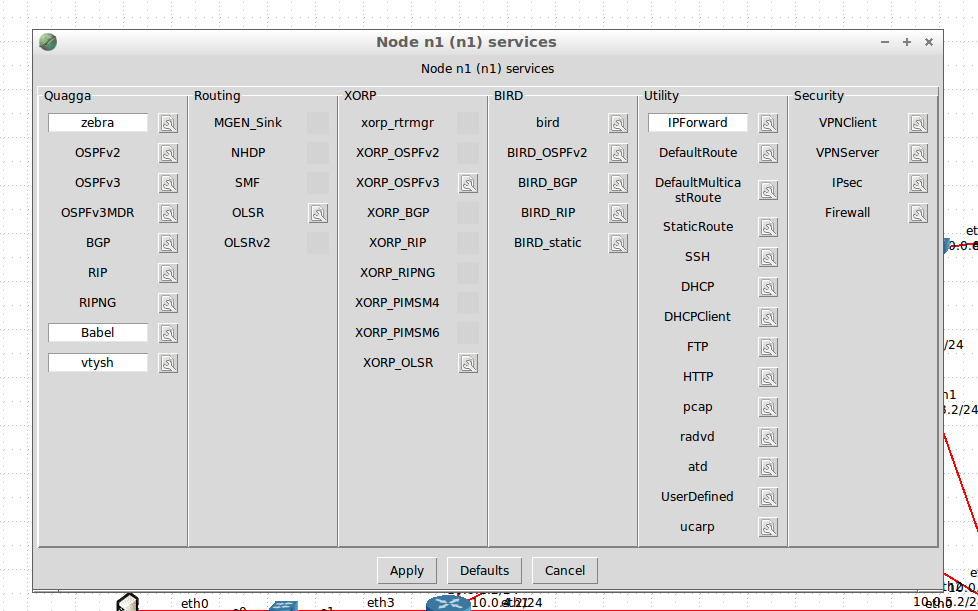
\includegraphics[scale=0.6]{\ImgPath/Ex4/Step1/servicesBabelenable.png}
\caption{Enable Service configuration}
\label{fig:2}
\centering
\end{figure}
%</mtag101>
%<*mtag102>
\begin{figure}[H]
\centering
\captionsetup{width=1\linewidth}
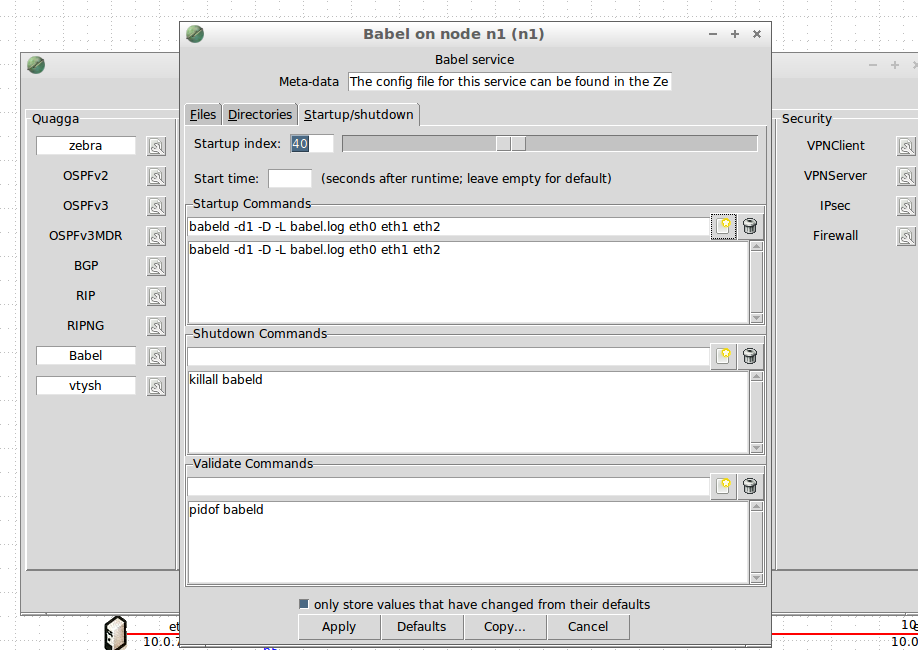
\includegraphics[scale=0.4]{\ImgPath/Ex4/Step1/babelStartup.png}
\caption{Babel daemon start up command}
\label{fig:3}
\centering
\end{figure}
%</mtag102>
%<*mtag103>
\begin{figure}[H]
\centering
\captionsetup{width=1\linewidth}
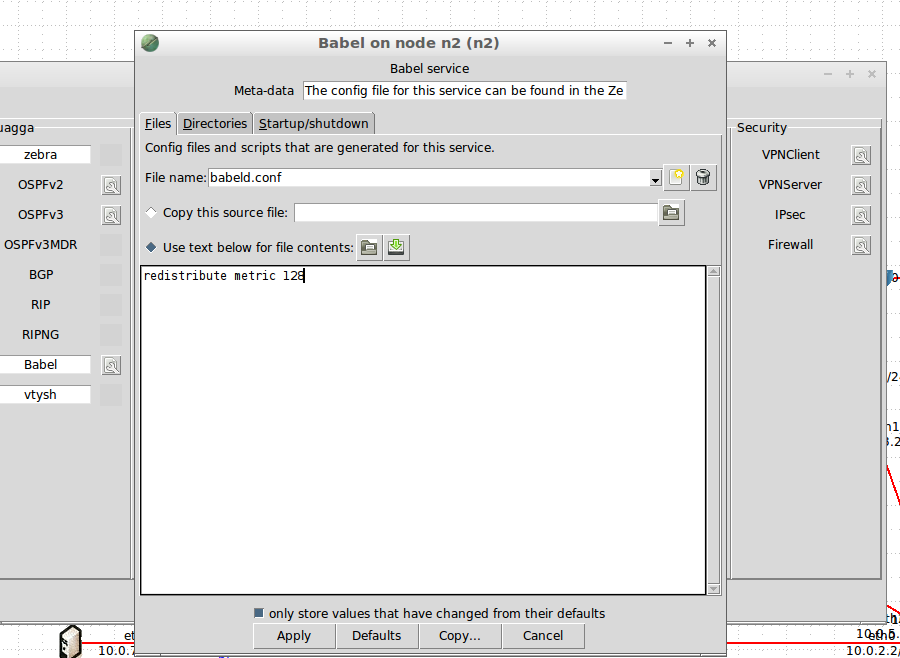
\includegraphics[scale=0.4]{\ImgPath/Ex4/Step1/redistribute.png}
\caption{Babel configuration, redistribute metric}
\label{fig:4}
\centering
\end{figure}
%</mtag103>
%<*mtag104>
\begin{figure}[H]
\centering
\captionsetup{width=1\linewidth}
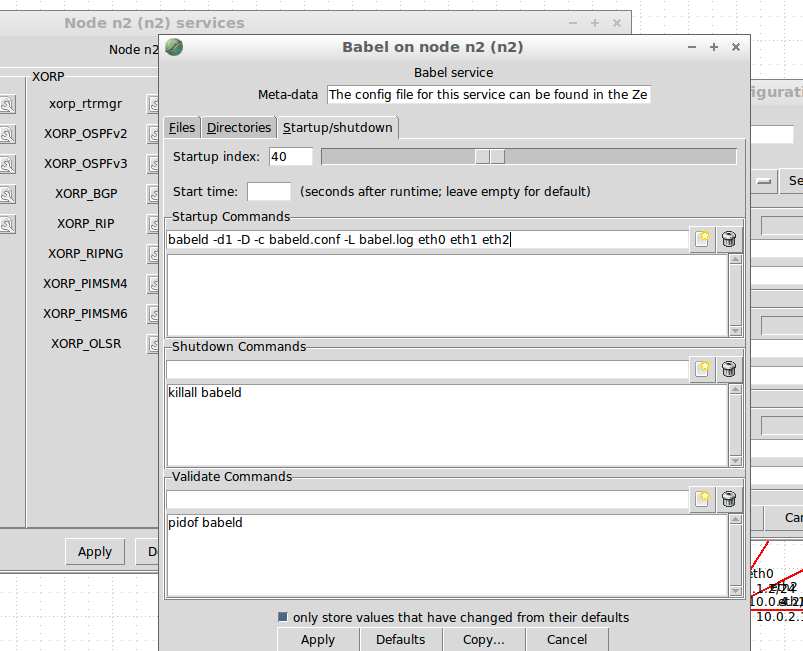
\includegraphics[scale=0.4]{\ImgPath/Ex4/Step1/babelN2config.png}
\caption{Babel startup command pointing to configuration file}
\label{fig:5}
\centering
\end{figure}
%</mtag104>
%<*mtag105>
\begin{figure}[H]
\centering
\captionsetup{width=1\linewidth}
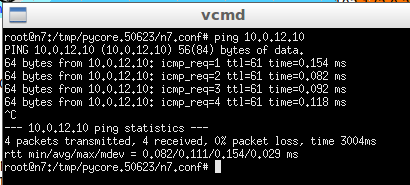
\includegraphics[scale=0.4]{\ImgPath/Ex4/Step1/wiredConnectivityTest.png}
\caption{Connectivity in Babel Wired Mesh Network}
\label{fig:6}
\centering
\end{figure}
%</mtag105>
%<*mtag106>
\begin{figure}[H]
\centering
\captionsetup{width=1\linewidth}
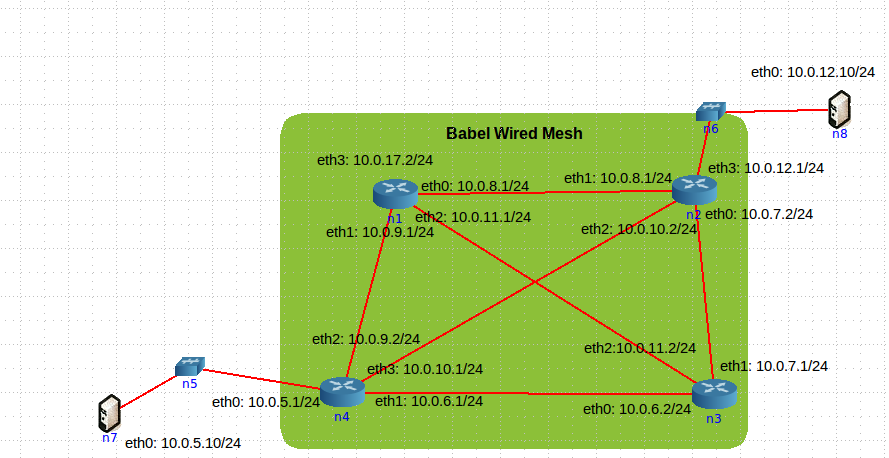
\includegraphics[scale=0.6]{\ImgPath/Ex4/Step1/babelwirednet-diagram.png}
\caption{Wired Babel Mesh Network}
\label{fig:Ex1-7}
\centering
\end{figure}
%</mtag106>
%====================Step2====================%
%<*mtag200>
\begin{figure}[H]
\centering
\captionsetup{width=1\linewidth}
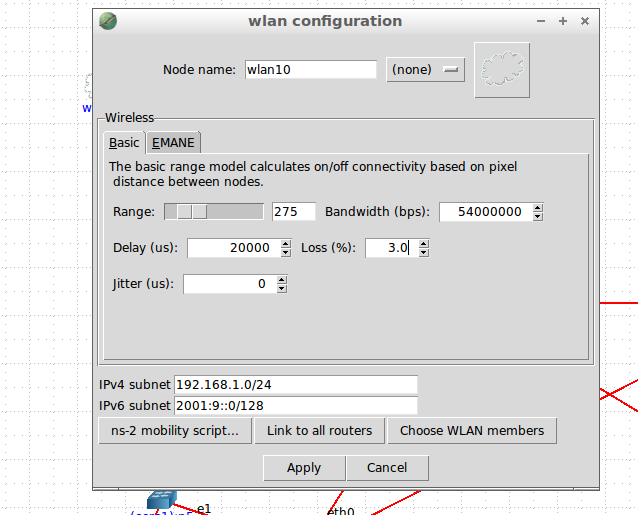
\includegraphics[scale=0.4]{\ImgPath/Ex4/Step2/wlanconfig.png}
\caption{Wireless Lan Configuration Tab}
\label{fig:7}
\centering
\end{figure}
%</mtag200>
%<*mtag201>
\begin{figure}[H]
\centering
\captionsetup{width=1\linewidth}
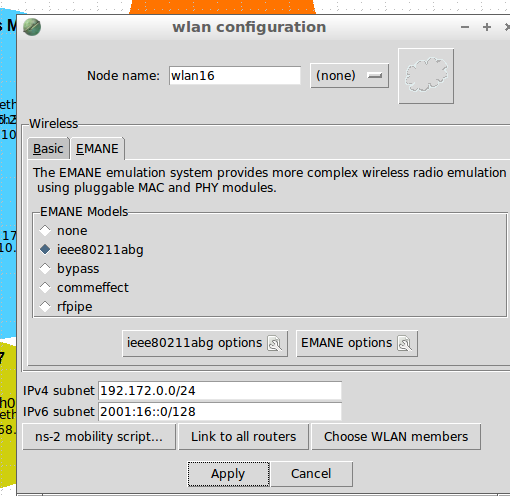
\includegraphics[scale=0.4]{\ImgPath/Ex4/Step2/emane.png}
\caption{Wireless Lan EMANE Configuration Tab}
\label{fig:8}
\centering
\end{figure}
%</mtag201>
%<*mtag202>
\begin{figure}[H]
\centering
\captionsetup{width=1\linewidth}
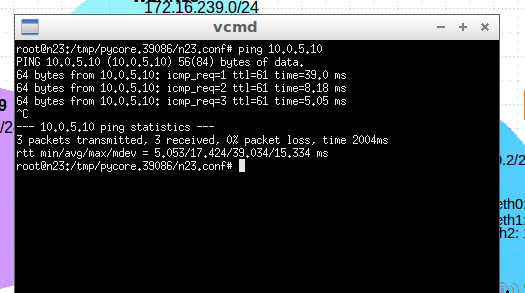
\includegraphics[scale=0.7]{\ImgPath/Ex4/Step2/pingWirlessClienttoWired.png}
\caption{Successful connectivity between wireless network and wired}
\label{fig:9}
\centering
\end{figure}
%</mtag202>
%<*mtag203>
\begin{figure}[H]
\centering
\captionsetup{width=1\linewidth}
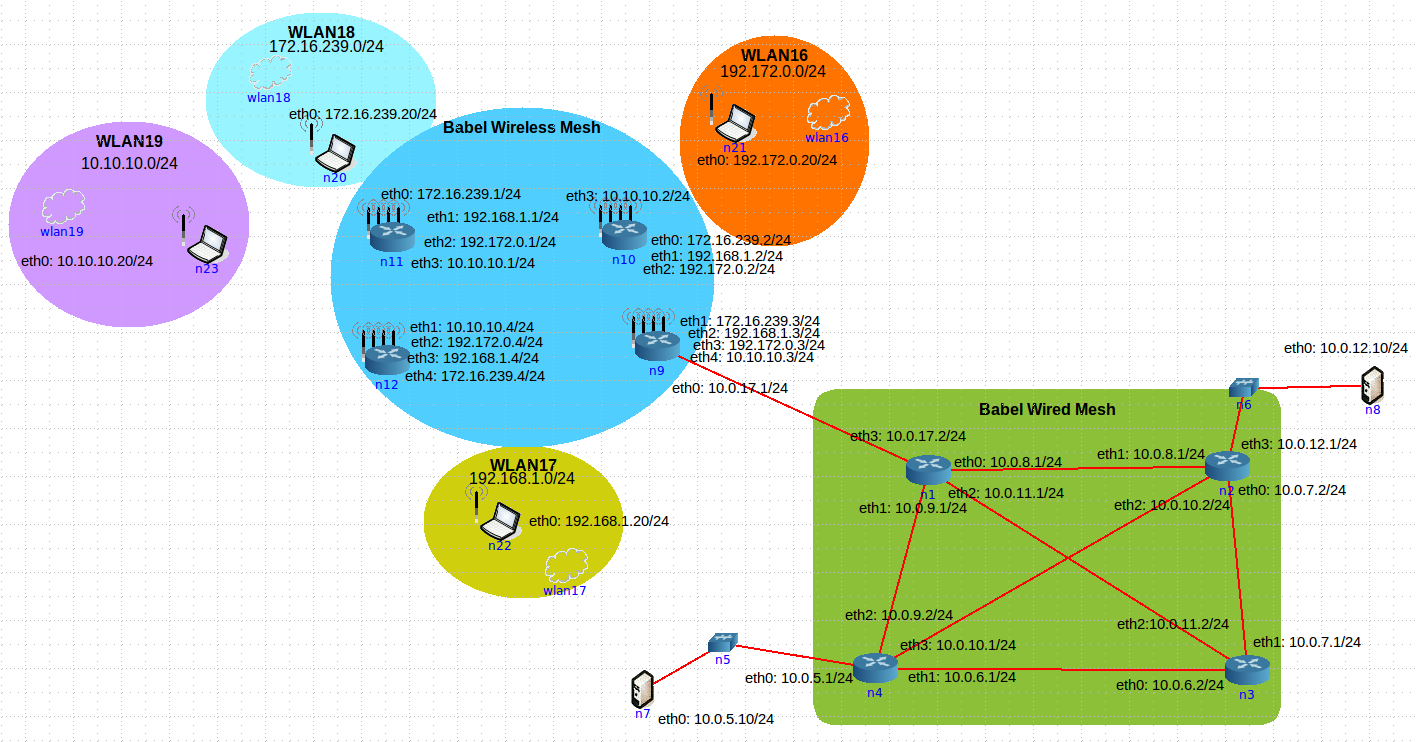
\includegraphics[scale=0.35]{\ImgPath/Ex4/Step2/wirelessandwirednet-diagram.png}
\caption{Added Wireless Messh Network}
\label{fig:10}
\centering
\end{figure}
%</mtag203>
%====================Step3====================%
%<*mtag300>
\begin{figure}[H]
\centering
\captionsetup{width=1\linewidth}
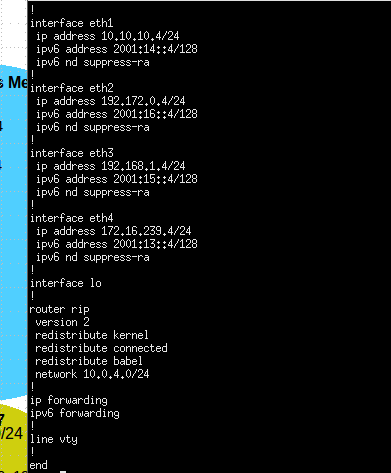
\includegraphics[scale=0.8]{\ImgPath/Ex4/Step3/n12RunningConfig.png}
\caption{Shows the RIP configuration for n12}
\label{fig:Ex3-1}
\centering
\end{figure}
%</mtag300>
%<*mtag301>
\begin{figure}[H]
\centering
\captionsetup{width=1\linewidth}
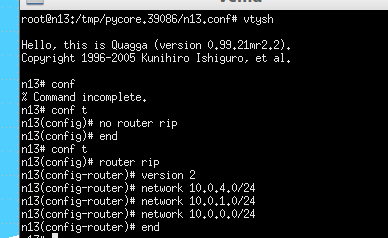
\includegraphics[scale=0.8]{\ImgPath/Ex4/Step3/n13RIPconfig.png}
\caption{Shows the RIP configuration for n13}
\label{fig:Ex3-2}
\centering
\end{figure}
%</mtag301>
%<*mtag302>
\begin{figure}[H]
\centering
\captionsetup{width=1\linewidth}
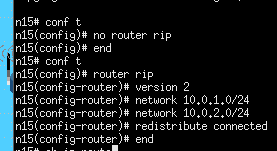
\includegraphics[scale=1.0]{\ImgPath/Ex4/Step3/n15RIPConf.png}
\caption{Shows the RIP configuration for n15}
\label{fig:Ex3-3}
\centering
\end{figure}
%</mtag302>
%<*mtag303>
\begin{figure}[H]
\centering
\captionsetup{width=1\linewidth}
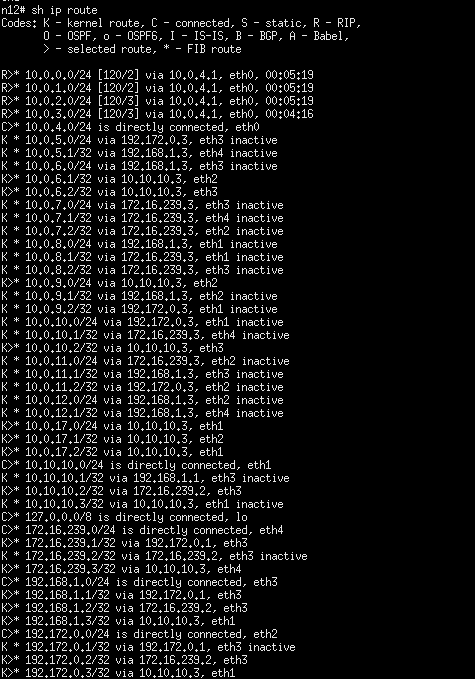
\includegraphics[scale=0.8]{\ImgPath/Ex4/Step3/shipRouteN12.png}
\caption{Show IP route on n12}
\label{fig:Ex3-4}
\centering
\end{figure}
%</mtag303>
%<*mtag304>
\begin{figure}[H]
\centering
\captionsetup{width=1\linewidth}
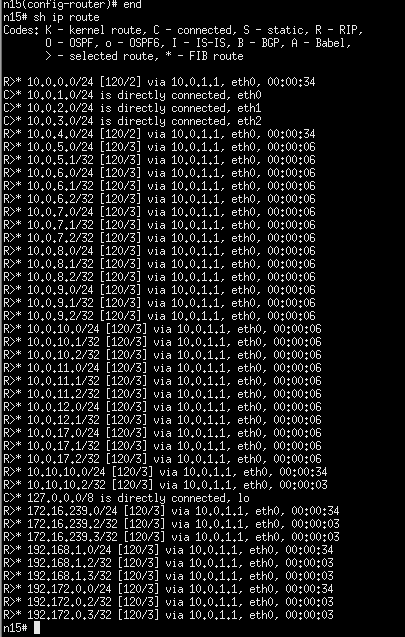
\includegraphics[scale=0.8]{\ImgPath/Ex4/Step3/n15Ship.png}
\caption{Show IP route on n15}
\label{fig:Ex3-5}
\centering
\end{figure}
%</mtag304>
%<*mtag305>
\begin{figure}[H]
\centering
\captionsetup{width=1\linewidth}
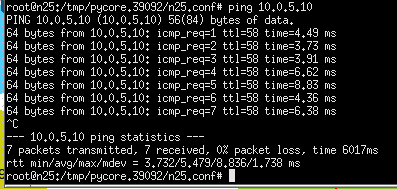
\includegraphics[scale=0.8]{\ImgPath/Ex4/Step3/pingFromRiptoWired.png}
\caption{Succesful ping from host on RIP network to host on Babel Wired Mesh Network}
\label{fig:Ex3-6}
\centering
\end{figure}
%</mtag305>
%====================Step4====================%
%<*mtag400>
\begin{figure}[H]
\centering
\captionsetup{width=1\linewidth}
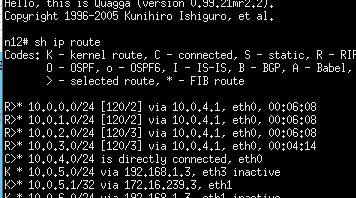
\includegraphics[scale=1.2]{\ImgPath/Ex4/Step4/n12StartingRoute.png}
\caption{Starting routing entry on N12 for network 10.0.5.0/24}
\label{fig:Ex4-1}
\centering
\end{figure}
%</mtag400>
%<*mtag401>
\begin{figure}[H]
\centering
\captionsetup{width=1\linewidth}
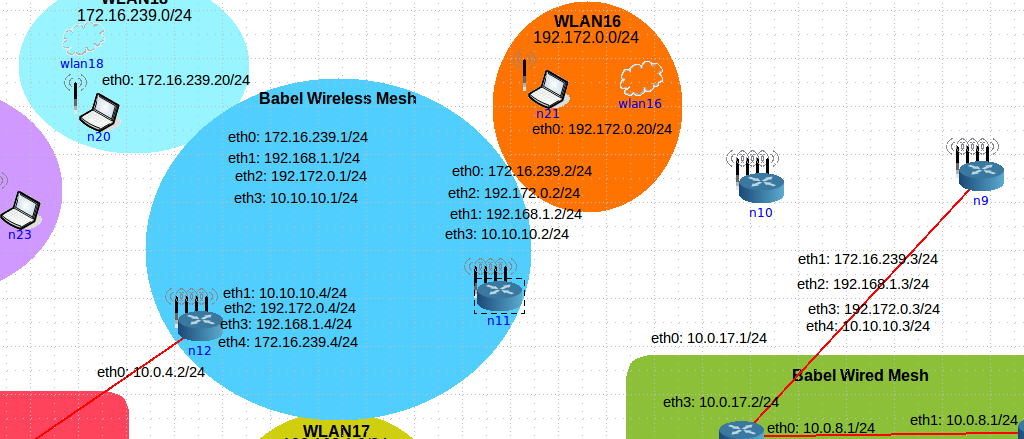
\includegraphics[scale=0.4]{\ImgPath/Ex4/Step4/movedNodes.png}
\caption{Starting routing entry on N12 for network 10.0.5.0/24}
\label{fig:Ex4-2}
\centering
\end{figure}
%</mtag401>
%<*mtag402>
\begin{figure}[H]
\centering
\captionsetup{width=1\linewidth}
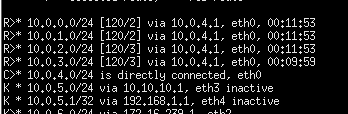
\includegraphics[scale=0.8]{\ImgPath/Ex4/Step4/afterChangingNodePosition.png}
\caption{After moving nodes around route entry on N12 for network 10.0.5.0/24 changed}
\label{fig:Ex4-3}
\centering
\end{figure}
%</mtag402>
%<*mtag403>
\begin{figure}[H]
\centering
\captionsetup{width=1\linewidth}
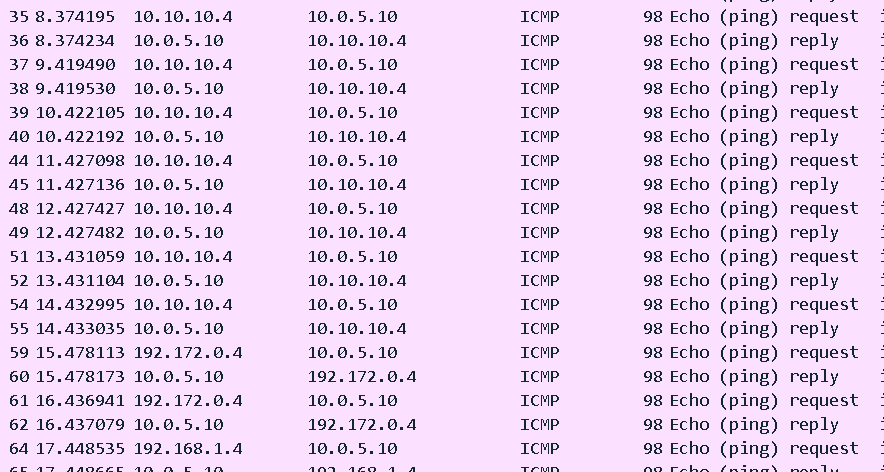
\includegraphics[scale=0.6]{\ImgPath/Ex4/Step4/wiresharkICMPsrc.png}
\caption{Src IP switching during ICMP request}
\label{fig:Ex4-4}
\centering
\end{figure}
%</mtag403>
